\chapter{Introduction}
\label{ch:Introduction}

Dans le cadre de notre ST4 \textit{Big Data et Santé}, nous avons choisi l'enseignement d'intégration en partenariat avec le service de radiologie de l'hôpital Henri Mondor. Notre projet consiste à développer un outil d'aide à la décision pour la détection du type de cancer du foie et la prédiction de la survie des patients.

\section{Données}

Notre approche repose donc sur des données anonymisées fournies par l'hôpital Henri Mondor, qui comprennent des données radiomiques, cliniques, et d'observations médicales. Ces données sont réparties dans plusieurs tableaux. Les patients sont identifiés par le couple \texttt{(patient\_num, classe\_name)}, où \texttt{patient\_num} est le numéro du patient et \texttt{classe\_name} est le type de cancer du foie. Les types de cancer du foie présents dans le dataset sont les suivants: CCK, CHC et Mixtes. De plus, on prend en compte différentes phases d'injections, dans \texttt{temps\_inj}, qui sont: artérielle, portale et veineuse et tardive, notées respectivement \texttt{ART, PORT, VEIN, TARD}. De plus, nous avons un set de données contenant des coupes de la tumeur, nous donnant des informations sur la taille et l'intérieur de la tumeur.

Voici donc des statistiques sur le dataset que nous avons utilisé:

\begin{figure}[H]
\centering
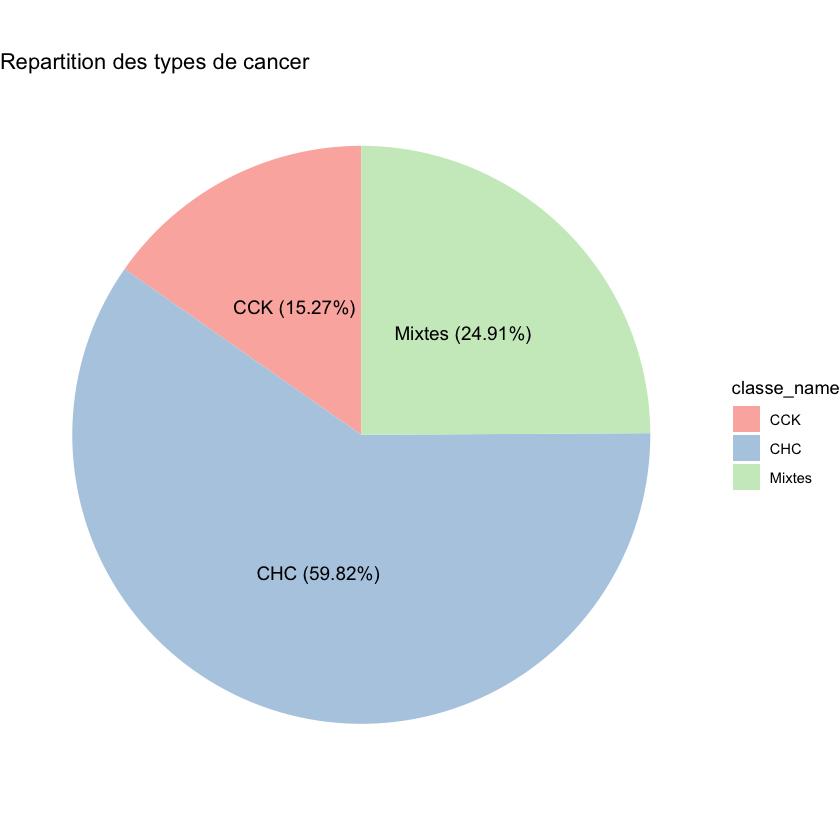
\includegraphics[width=0.23\textwidth]{img/repartition-type.png}
\caption{Répartition des types de cancer du foie dans le dataset}
\end{figure}

\begin{figure}[H]
\centering
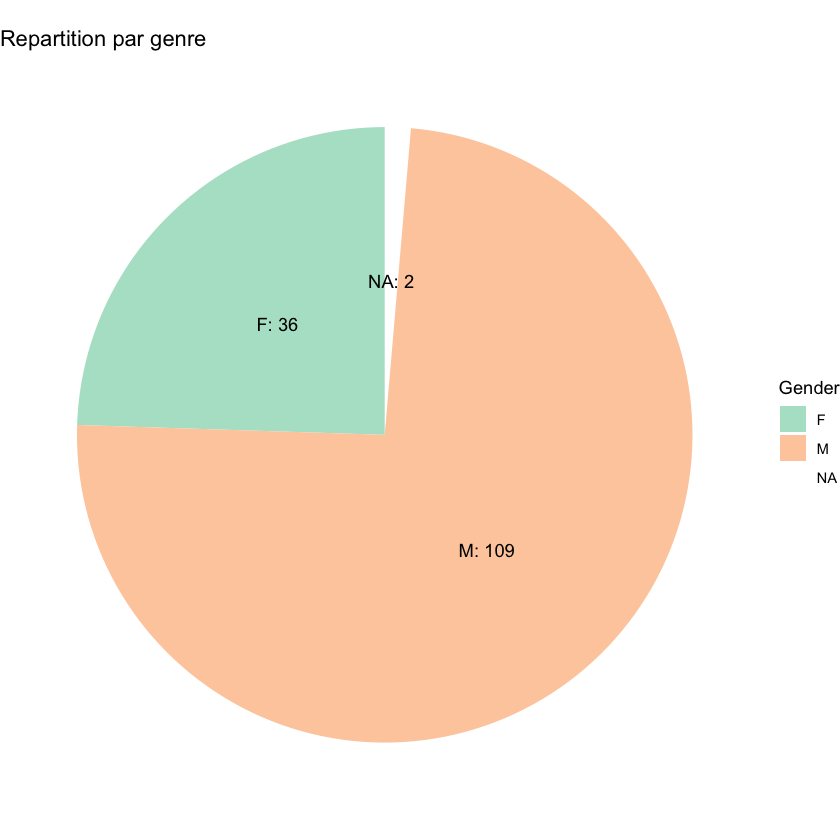
\includegraphics[width=0.23\textwidth]{img/repartition-genre.png}
\caption{Répartition des genres dans le dataset}
\end{figure}

\begin{figure}[H]
\centering
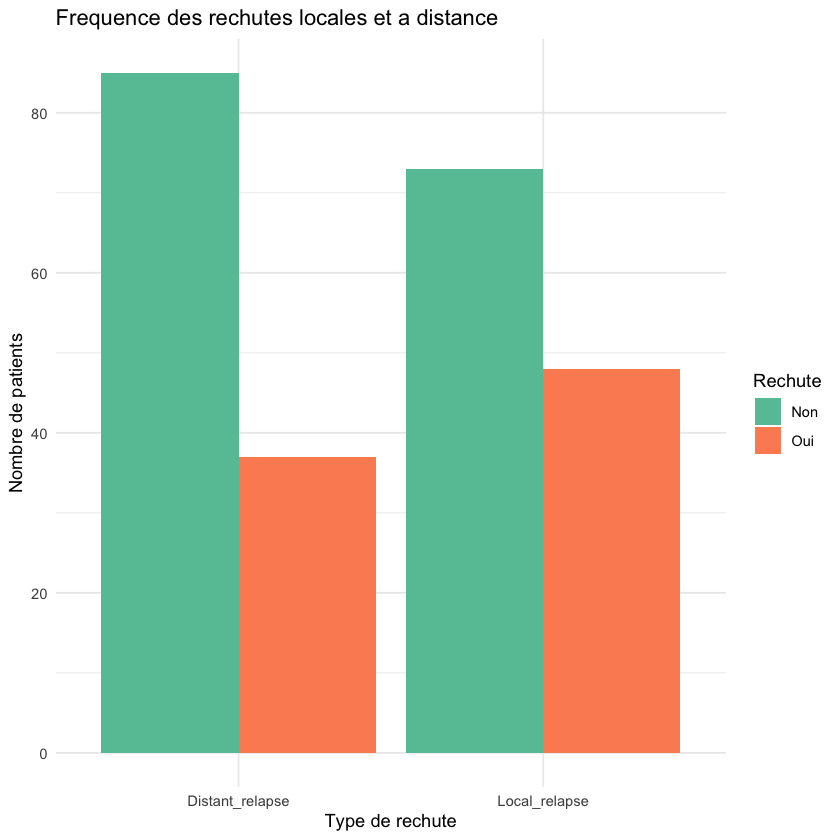
\includegraphics[width=0.23\textwidth]{img/freq-rechute.png}
\caption{Fréquence de rechute des patients, par type de rechute}
\end{figure}

\begin{figure}[H]
\centering
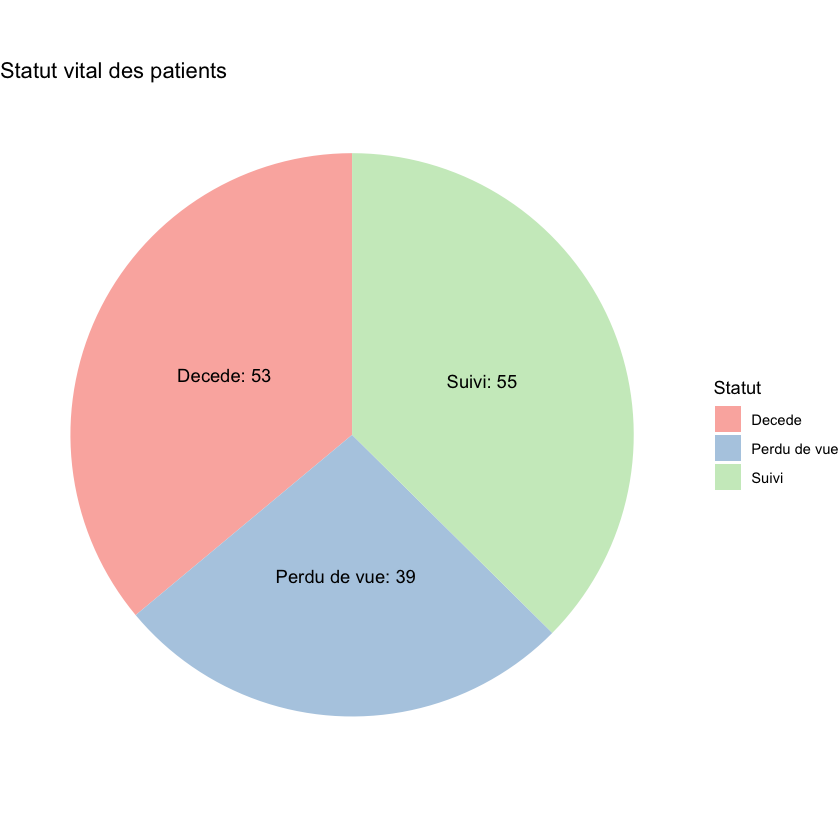
\includegraphics[width=0.23\textwidth]{img/statut-vital.png}
\caption{Statut vital des patients}
\end{figure}

\begin{figure}[H]
\centering
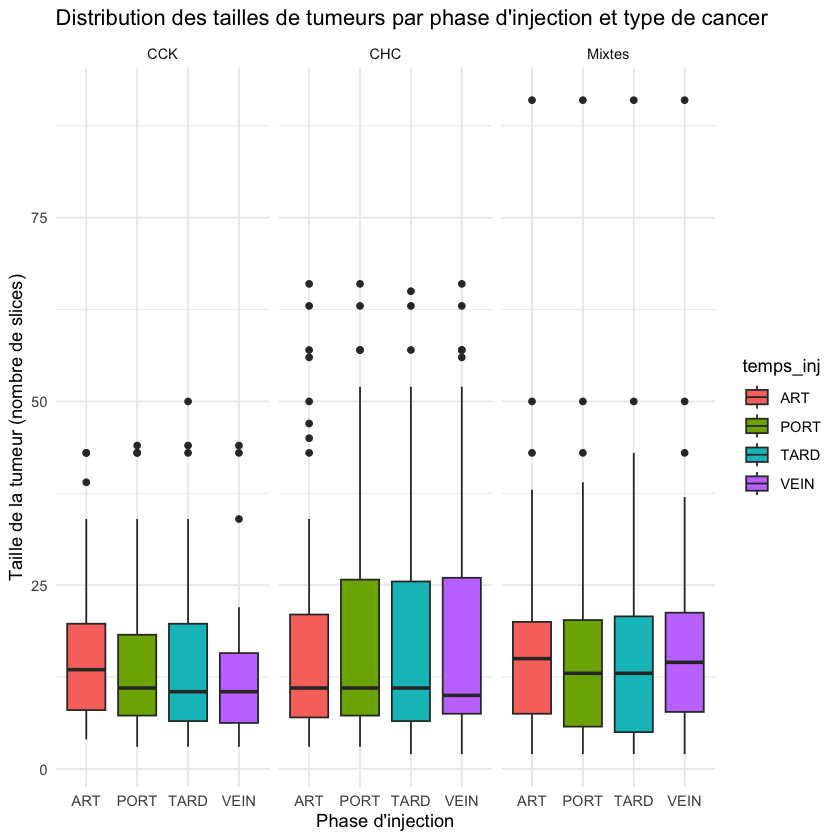
\includegraphics[width=0.23\textwidth]{img/taille-cancer.png}
\caption{Distribution de la taille des cancers par type de cancer et par phase}
\end{figure}

En tout, nous avons un dataset de 148 patients.

On remarque que le dataset est déséquilibré, contenant une majorité de patients atteints de CHC, et une minorité de patients atteints de CCK. De plus, on remarque que la majorité des patients sont des hommes.
